\documentclass[aps,prl,reprint,amsmath,amssymb,floatfix]{revtex4-2}
\usepackage{graphicx,bm,amsmath,amssymb,physics}
\usepackage[colorlinks=true,linkcolor=blue,citecolor=blue,urlcolor=blue]{hyperref}
\graphicspath{{Figures/}}
\newcommand{\UK}{U_{\mathrm K}}
\newcommand{\UI}{U_{\mathrm I}}
\newcommand{\EN}{E_{\mathcal N}}
\newcommand{\Psym}{P_{\mathrm{ring}}}
\begin{document}
\title{Extracting Operational Entanglement from a Noise-Protected Many-Body System}
\author{Bhavay Tyagi}
\email{btyagi@uh.edu}
\affiliation{Department of Physics, University of Houston, Houston, Texas 77204, USA}
\author{Eric R. Bittner}
\affiliation{Department of Physics, University of Houston, Houston, Texas 77204, USA}
\author{Kevin E. Bassler}
\affiliation{Department of Physics, University of Houston, Houston, Texas 77204, USA}
\date{\today}
\begin{abstract}
Can a noisy interacting system generate entanglement that remains useful at long times? We show that collective dephasing protects an entangled many-body attractor reached from an unentangled product state in a kicked Ising ring. Coherent operations within each half of the ring extract a physical pair that teleports an unknown qubit with greater than $90\%$ fidelity, heralded with an average probability of $1/192$. As a result, the surviving entanglement serves as a viable operational resource. For imperfect correlations, our finite-time simulations show correlation-dependent survival of the chosen decoder's teleportation advantage.
\end{abstract}
\maketitle

We traditionally treat noise as the enemy of coherence, and counter it either by isolating the system better or by correcting its errors~\cite{Acharya2023}. A complementary route asks what the environment can actually \emph{see}. Figure~\ref{fig:model} (a) illustrates this distinction. Independent noise channels resolve the coupled spin component at each site, whereas a collective field couples only to their sum. Spatial correlations in the environment therefore determine how well it can distinguish different spin configurations. Decoherence-free subspaces and noiseless subsystems exploit collective coupling to preserve quantum information~\cite{Zanardi1997,Lidar1998,Knill2000}. Correlated dephasing has also been measured in trapped-ion, superconducting and silicon-spin devices~\cite{Monz2011,vonLupke2020,Yoneda2023}. Our earlier work showed that a shared correlated environment can synchronize two coupled spins~\cite{Tyagi2024} and coupled quantum oscillators~\cite{Bittner2025jcp}. These studies explored how environmental correlations can organize collective quantum dynamics. We now carry this question into an interacting many-body system. Can a correlated environment protect entanglement that the system generates intrinsically, starting from an unentangled state? What fixes its surviving amount, and can it be used to perform a quantum task?

Strong symmetries also organize dissipative dynamics into invariant sectors~\cite{BucaProsen2012}. For unital channels with non-Abelian on-site symmetries, maximally mixed invariant-sector states can be entangled and have distillable entanglement~\cite{Moharramipour2024}. These results motivate a concrete question for spatial symmetries: can a driven ring prepare such a mixed resource from a product state, and can operations on physical spins expose its usefulness? The extraction question is related to localizable entanglement, which studies entanglement localized between spins by measurements on the others~\cite{Popp2005}. Here we allow coherent gates within each half of the ring and specify one heralded filter, without optimizing over all such operations.

\begin{figure}[tbp]
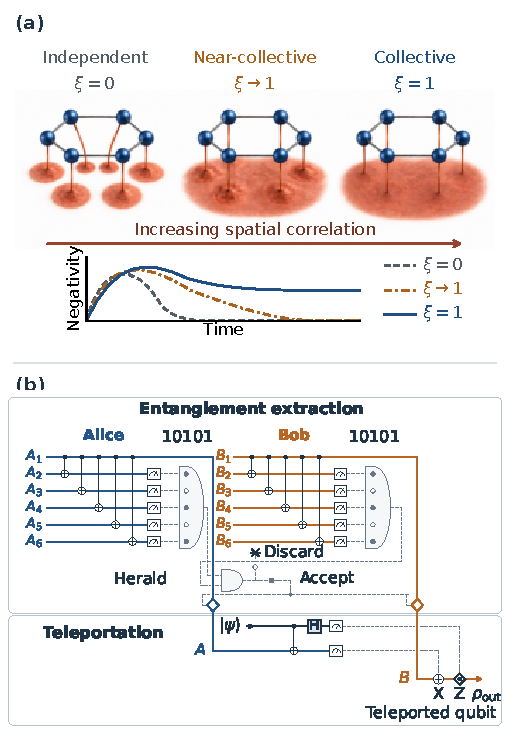
\includegraphics[width=\linewidth]{combined_opening.pdf}
\caption{\label{fig:model} (a) Schematic comparison of independent and collective dephasing. A collective environment cannot distinguish spin configurations with the same total magnetization. Blue spins represent the interacting ring, and red regions depict its dephasing environment. The schematic negativity curves illustrate entanglement survival as $\xi\rightarrow1$. (b) Circuit representing the full protocol. In the extraction phase, Alice and Bob apply local CNOT gates and measurements to their halves of the spin chain. They retain the resource pair ($A$ and $B$) only if each obtains the predetermined classical record $10101$. The teleportation phase uses this extracted pair to teleport an unknown input qubit $\ket{\psi}$ via Bell-state measurement and Pauli corrections to yield $\rho_{\text{out}}$. The ring-and-environment artwork in (a) was generated and edited with the built-in \texttt{image\_gen} tool; labels, schematic curves and circuit were composed separately.}
\end{figure}


\emph{In this Letter} we connect spatial-symmetry-restricted noisy dynamics to a physical teleportation resource in a driven Ising ring~\cite{Bertini2018}. The protecting transformations permute ring sites, rather than acting as the on-site symmetry considered in Ref.~\cite{Moharramipour2024}. Starting from a uniform product state, interactions generate entanglement. Collective dephasing preserves the ring-symmetric sector containing that input, and the driven dynamics approaches a maximally mixed density within this sector. For twelve spins, a fixed decoder confined to the two separate halves extracts an entangled pair of physical spins and uses it for teleportation above the classical fidelity benchmark. Figure~\ref{fig:model}(b) shows the extraction and subsequent task. The contribution is this explicit preparation-to-task connection, with separately quantified accepted-pair fidelity and extraction probability; it does not require every state in the sector to be unchanged by noise.

\emph{Model and preparation.}---The one-period quantum channel $\mathcal M_\xi$ applies an Ising layer, a transverse kick, and accumulated dephasing, in that order.
\begin{align}
\UI&=\exp\!\left[-i\left(J\sum_{j=1}^{L}\sigma_j^z\sigma_{j+1}^z+h\sum_{j=1}^{L}\sigma_j^z\right)\right],\nonumber\\
\UK&=\exp\!\left[-ib\sum_{j=1}^{L}\sigma_j^x\right],\nonumber\\
\rho_{t+1}&=\mathcal M_\xi[\rho_t]\nonumber\\
&\equiv e^{\mathcal D_\xi}\!\left(\UK\UI\rho_t\UI^\dagger\UK^\dagger\right).
\label{eq:map}
\end{align}
The boundary is periodic, $\sigma^z_{L+1}=\sigma^z_1$, and one period is the unit of time. This well-studied spin chain combines local interactions with periodic driving and supplies a direct gate decomposition. At its self-dual points, \emph{space-time} duality permits exact calculations of selected spectral and entanglement observables of the coherent dynamics~\cite{Bertini2018,Bertini2019}. We set $J=\pi/4$, $b=-\pi/4$, and $h=1$, placing the coherent evolution at a \emph{dual-unitary point}. This is the model point studied here. The stationary projector below follows from spatial symmetry and unitality; its attraction additionally uses the finite-size algebraic certificate in End matter A. We do not infer robustness away from these parameters from dual unitarity. We prepare the uniform product state $\rho_0=(\ket{+}\!\bra{+})^{\otimes L}$, where $\ket{+}=(\ket0+\ket1)/\sqrt2$.

We describe the accumulated dephasing by the Lindblad generator~\cite{Breuer2007},
\begin{equation}
\mathcal D_\xi[\rho]=\gamma\sum_{i,j=1}^{L}\Xi_{ij}\left(\sigma_i^z\rho\sigma_j^z-\tfrac12\{\sigma_j^z\sigma_i^z,\rho\}\right).
\label{eq:noise}
\end{equation}
Here $\sigma_i^z$ are the local dephasing operators and $\Xi_{ij}=(1-\xi)\delta_{ij}+\xi$ is the noise-correlation matrix. The covariance eigenvalues give the physical range
$-1/(L-1)\le\xi\le1$ and leave only one active collective noise mode at
$\xi=1$ (see End matter~C). For $0\le\xi\le1$, each spin is subject to a shared noise channel and an independent local noise channel. Increasing $\xi$ increases the shared contribution while keeping the total noise strength at each spin fixed. At $\xi=0$, the noise channels are independent; at $\xi=1$, a single collective noise channel acts on all spins. The allowed negative values describe anticorrelated noise. The channel $e^{\mathcal D_\xi}$ is obtained exactly by averaging Gaussian white phase noise applied after the coherent layers. All trajectories reported here use the dephasing rate $\gamma=0.1$.

To quantify the entanglement generated during evolution, we divide the ring into two contiguous equal halves and calculate the logarithmic negativity~\cite{Vidal2002},
\begin{equation}
\EN(t)=\ln\|\rho_t^{T_A}\|_1.
\label{eq:negativity}
\end{equation}
A positive value certifies entanglement between the two halves. We use the natural logarithm. The product input has $\EN(0)=0$.

\begin{figure}[!t]
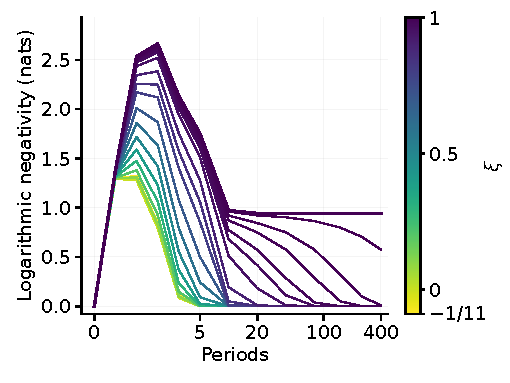
\includegraphics[width=\linewidth]{negativity_L12_correlations.pdf}
\caption{\label{fig:negativity}Correlation dependence of generated entanglement for twelve spins over the twenty correlations used in Fig.~\ref{fig:dynamics}. The initial state is the uniform product input $(\ket{+}\!\bra{+})^{\otimes12}$. Logarithmic negativity is in natural-log units. Markers give the thirteen calculated times $0,1,2,3,4,5,10,20,40,80,150,250,400$; connecting lines are visual guides. The time axis is linear through five Floquet periods and logarithmic thereafter. Representative near-collective curves are identified by marker shape and legend.}
\end{figure}

\emph{Results.}---Starting from $\rho_0$, interactions generate entanglement between the two halves. Figure~\ref{fig:negativity} gives logarithmic negativity at thirteen sampled times through $400$ periods. The initial buildup is followed by decay whose late-time behavior depends strongly on the noise correlations. Under collective dephasing, the twelve-spin trajectory approaches the entangled stationary state. Near the collective limit the early buildup is similar, while entanglement persists longer over the observed interval as $\xi\rightarrow1$. These finite-time comparisons concern the stated model and noise covariance. They do not establish a device preparation rate or a universal protection time for imperfect correlations.

\begin{figure*}[t]
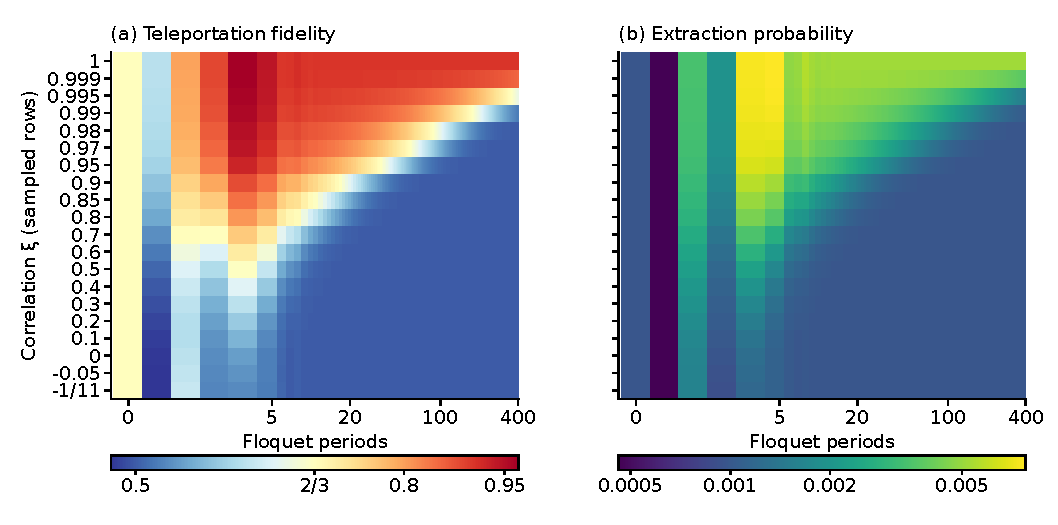
\includegraphics[width=\textwidth]{xi_resource_L12_all20.pdf}
\caption{\label{fig:dynamics}Correlation dependence of entanglement extraction and teleportation for twelve spins. The twenty equally spaced rows have nonuniform correlation spacing: $\xi=-1/11,\allowbreak -0.05,\allowbreak 0,\allowbreak 0.1,\allowbreak 0.2,\allowbreak 0.3,\allowbreak 0.4,\allowbreak 0.5,\allowbreak 0.6,\allowbreak 0.7,\allowbreak 0.8,\allowbreak 0.85,\allowbreak 0.9,\allowbreak 0.95,\allowbreak 0.97,\allowbreak 0.98,\allowbreak 0.99,\allowbreak 0.995,\allowbreak 0.999,\allowbreak 1$. (a) Fixed-decoder conditional teleportation fidelity, with color centered on the classical benchmark $2/3$, and (b) heralding probability on a logarithmic color scale. The input and parameters are those of Fig.~\ref{fig:negativity}. Each constant-color time cell represents one of the $401$ integer times from $0$ through $400$ periods; the cell boundaries are at half-integer times. Time axes are linear through five Floquet periods and logarithmic thereafter, so the displayed cell widths are unequal.}
\end{figure*}

The Lindblad generator $\mathcal D_\xi$ describes the dephasing layer, while $\mathcal M_\xi$ in Eq.~\eqref{eq:map} describes the full period. For collective dephasing, $\xi=1$, the stationary state here satisfies $\mathcal D_1[\rho_\infty]=0$ and $\mathcal M_1[\rho_\infty]=\rho_\infty$. Let $D_L$ comprise the ring's $L$ rotations and $L$ reflections, represented by spin permutations $U(g)$. Its group average gives
\begin{equation}
\Psym=\frac{1}{2L}\sum_{g\in D_L}U(g),
\quad N_L=\Tr\Psym,\quad
\rho_\infty=\frac{\Psym}{N_L}.
\label{eq:target}
\end{equation}
Here $\Psym$ is the orthogonal projector onto $\mathcal S$, the subspace of spin states unchanged by every rotation and reflection of the ring, and $N_L=\dim\mathcal S$. Thus $\rho_\infty$ is maximally mixed on $\mathcal S$, which contains the uniform product input. Both coherent layers and the collective jump $\sum_j\sigma_j^z$ preserve support in $\mathcal S$. Each layer separately leaves $\rho_\infty$ unchanged. Preservation of this sector does not imply that arbitrary supported states or coherences remain unchanged.

End matter A establishes convergence from every state supported on $\mathcal S$ at the stated parameters for $L=12$. Within that sector, the limiting density is independent of the initial supported state; it is not a globally unique attractor for arbitrary ring inputs. Departures from perfectly collective noise remove this support protection. Although the averaged channel remains covariant under the dihedral ring transformations, its individual noise operators need not preserve $\mathcal S$. The ideal target ceases to be stationary for every allowed $\xi<1$; this alone is not an assertion about the long-time usefulness of a different state.

A nonzero logarithmic negativity confirms entanglement in the stationary state, but does not by itself specify how to access this resource. Here, accessing the resource means using local operations within the two halves to extract an entangled pair of physical spins suitable for a quantum task. We use this pair for quantum teleportation, whose fidelity quantifies how accurately an unknown quantum state can be transferred between the two halves. We extract the pair by probabilistic local filtering~\cite{Teleportation1999}. In each half of $m=L/2$ spins, select the alternating string $a=0101\cdots$ and its complement $\bar a$. The operator for a successful local outcome is given by
\begin{equation}
K=\ket0\bra a+\ket1\bra{\bar a}.
\label{eq:decoder}
\end{equation}
Alice and Bob each have access to one half of the spin chain, with six spins in each half for the twelve-spin system considered here. Within each half, apply five controlled-NOT gates, using the first spin as the control and each of the other five spins as a target. Measure the five target spins in the computational basis, leaving the first spin unmeasured. The selected strings, for six spins, $010101$ and $101010$ both produce the measurement record $10101$, leaving the retained spin in $0$ and $1$, respectively. Since the measurement does not distinguish these two configurations, their coherence is preserved in the retained spin. Alice and Bob communicate their measurement outcomes and keep the retained pair only if each obtains the predetermined record $10101$. All gates act within the individual halves, so the protocol extracts entanglement already present between them.

For a ring state $\rho_t$, the unnormalized pair, success probability, and conditional pair are
\begin{equation}
\sigma_t=(K\otimes K)\rho_t(K^\dagger\otimes K^\dagger),\quad
p_t=\Tr\sigma_t,\quad r_t=\sigma_t/p_t.
\label{eq:pair}
\end{equation}
For the twelve-spin target, the accepted pair is
\begin{equation}
r_\infty=\frac67\ket{\Phi^+}\!\bra{\Phi^+}+\frac17\ket{\Psi^+}\!\bra{\Psi^+},\qquad p_\infty=\frac1{192},
\label{eq:pair12}
\end{equation}
with $\ket{\Phi^+}=(\ket{00}+\ket{11})/\sqrt2$ and $\ket{\Psi^+}=(\ket{01}+\ket{10})/\sqrt2$. The Bell overlap $f\equiv \bra{\Phi^+}r_\infty\ket{\Phi^+}=6/7$. The overlap is the weight of the desired maximally entangled state $\ket{\Phi^+}$ in the accepted pair. For the twelve-spin steady state under collective dephasing, $\xi=1$, the standard teleportation measurement and corrections yield the fidelity $F$, averaged uniformly over all pure input qubits~\cite{Teleportation1999}
\begin{equation}
F=\frac{2f+1}{3}=\frac{19}{21}\simeq90.48\%>\frac23.
\label{eq:fidelity}
\end{equation}
This fidelity measures the average overlap of Bob's output with the unknown input state. Its value exceeds the classical limit $2/3$ achievable without shared entanglement, so the accepted pair provides a useful teleportation resource. The extraction succeeds with probability $p_\infty=1/192$. Alice and Bob learn whether extraction has succeeded from their local measurement records before the unknown input is supplied. They can therefore repeat the ring preparation and extraction independently until an accepted pair is ready, requiring $192$ preparations on average. The fidelity characterizes the quality of these accepted pairs, while the success probability determines how often they are obtained. This protocol demonstrates access to the resource without optimizing its extraction yield. 
%At sixteen spins the same target-state construction gives $F=25/27$ with $p=1/2000$.

{\it Discussion and Conclusions.}---Figure~\ref{fig:negativity} tracks entanglement generation and survival, while Fig.~\ref{fig:dynamics} evaluates the specified extraction protocol at every integer period. Its useful-time set is defined by conditional fidelity $F_t>2/3$, with the corresponding probability $p_t$ determining the extraction yield. Using a numerical threshold $F_t>2/3+10^{-10}$, the sampled useful integer times are $2$ through $178$ at $\xi=0.99$, whereas at $\xi=0.999$ the advantage persists from period $2$ through the end of the run at $400$. The latter observation is right-censored; no later loss or infinite-time advantage is inferred. These examples do not assert that the useful-time set is a single interval for all parameters.

For imperfect correlations, the chosen pair can lose its teleportation advantage while the ring remains entangled. For example, at $\xi=0.995$ and period $400$, the saved data give $\EN\simeq0.00989$ but $F\simeq0.6426<2/3$, with $p\simeq0.00148$. This concerns the fixed decoder and does not rule out other uses of the remaining entanglement. The observed correlation dependence is a finite-time result; we make no asymptotic claim here for imperfect noise, including the singular anticorrelated endpoint.

Note that the extraction requires local controlled-NOT gates and measurements within each half, followed by communication of their outcomes. During these operations, we assume that the driven and noisy ring evolution is suppressed and that the gates and measurements are ideal. In an implementation, gate and readout errors can change both the fidelity and success probability, while the durations of preparation, gates, readout and communication determine how long each attempt takes. Together with the small success probability, these durations set how often an accepted pair can be prepared; that rate requires a specified implementation and is not determined here. Repeated attempts assume independent resets. After a successful extraction, holding the pair until the input arrives is also idealized: the ring-symmetry argument does not automatically protect the extracted two-spin state against subsequent uncontrolled noise.

We show that collective dephasing protects entanglement generated by interactions from an initially unentangled product state. In the twelve-spin ring, collective noise preserves the ring-symmetric sector, within which the driven dynamics approaches an entangled stationary density. This density is unchanged by each coherent layer and by collective dephasing; preservation of the sector does not imply invariance of every supported state. A fixed decoder acting separately within the two halves extracts a physical pair that implements teleportation with uniform-input average fidelity $19/21$ and heralding probability $1/192$. The fidelity characterizes the quality of the accepted pairs, while the probability determines their extraction yield; their physical production rate depends on the implementation. The example connects a symmetry-protected many-body stationary state to a concrete quantum-information task and distinguishes persistent entanglement from the yield of an accessible resource.

\begin{acknowledgments}
\emph{Acknowledgements.}---This work was supported by the National Science Foundation (CHE-2404788) and the Robert A. Welch Foundation (E-1337). GPT-6-Astra assisted with earlier numerical calculations, extraction-protocol suggestions and manuscript editing. GPT-6.1 Sol assisted with the present manuscript revision and checks in separate contexts; Codex (GPT-6) coordinated the current review and integration. The authors take full responsibility for the content.
\end{acknowledgments}

\emph{Data availability.}---
The numerical calculations are retained in a private GitHub repository.

\bibliographystyle{apsrev4-2}
\bibliography{References_revision_2}

\clearpage
\section*{End matter}
\paragraph*{A. Symmetry-selected stationary state and attraction.}
Here $J^\alpha=\tfrac12\sum_j\sigma_j^\alpha$, $\gamma>0$, $\sin(2b)\ne0$, and the longitudinal field is uniform. We distinguish stationarity from convergence for the map in Eq.~\eqref{eq:map}.

\emph{1. Peripheral operators.} Write $\mathcal E=e^{\mathcal D_1}$ and $U_F=\UK\UI$. Suppose $\mathcal M_1X=\lambda X$ with $|\lambda|=1$, and set $Y=U_FXU_F^\dagger$. Unitary invariance and dephasing contraction give $\|X\|_2=\|\mathcal E(Y)\|_2\le\|Y\|_2=\|X\|_2$. In a total-$z$ eigenbasis, $\mathcal E$ strictly contracts every block connecting unequal magnetizations and leaves the other blocks unchanged. Equality therefore gives $\mathcal E(Y)=Y=\lambda X$, so $[J^z,Y]=[J^z,X]=0$. Conjugating the latter relation by $U_F$, and using $[\UI,J^z]=0$, gives $[\UK J^z\UK^\dagger,X]=0$. Since $\UK J^z\UK^\dagger=\cos(2b)J^z-\sin(2b)J^y$ and $\sin(2b)\ne0$, $X$ commutes with all three collective spins. It then commutes with $\UK$, leaving $\UI X\UI^\dagger=\lambda X$. Conversely, those conditions imply the peripheral relation. Thus\begin{align}
\operatorname{Fix}(\mathcal M_1)&=\{J^x,J^y,J^z,\UI\}',\nonumber\\
\operatorname{Per}_\lambda(\mathcal M_1)&=\{X:[X,J^{x,y,z}]=0,\ \UI X\UI^\dagger=\lambda X\}.
\label{eq:algebra}
\end{align}
A prime denotes the operators commuting with the listed generators. The highest-$J^z$ eigenspace is one dimensional, spanned by the fully polarized vector $v=\ket{0\cdots0}$. Thus $[J^z,X]=0$ implies $Xv=cv$. Since $\UI v$ is a phase times $v$, the peripheral relation forces $c=0$ whenever $\lambda\ne1$.

\emph{2. Convergence within the supported sector.} The initial density obeys $\Psym\rho_0\Psym=\rho_0$. Assume the fixed algebra restricted to $\mathcal S$ is scalar; step 3 establishes this at the listed sizes. Unitality then makes $\Psym/N_L$ the unique stationary density in this sector. For a peripheral $X$, the Schwarz inequality for the restricted unital completely positive channel gives $\mathcal M_1(X^\dagger X)-\mathcal M_1(X)^\dagger\mathcal M_1(X)\succeq0$. Trace preservation and $|\lambda|=1$ make the trace of this positive difference zero, so $X^\dagger X$ is fixed. Scalarity gives $X^\dagger X=c\mathbb I_{\mathcal S}$; for nonzero $X$, $c>0$ and $X$ is invertible on $\mathcal S$. For $\lambda\ne1$, step 1 instead gives $Xv=0$, with $v\in\mathcal S$, a contradiction. Finally, the Hilbert--Schmidt contraction makes all powers of $\mathcal M_1$ bounded, excluding nontrivial Jordan blocks at unit-modulus eigenvalues. All remaining spectral components decay. Hence every supported density converges ordinarily to Eq.~\eqref{eq:target}, without time averaging.

\emph{3. Finite-size certificate.} At $J=\pi/4$, the periodic Ising layer is $\UI=e^{-i\pi L/4}R e^{-i2hJ^z}$, where $R=(-1)^{n_{\mathrm{DW}}/2}$ and $n_{\mathrm{DW}}$ counts the even number of domain walls. The algebra generated by $J^{x,y,z}$ and $\UI$ therefore contains $R$, the spectral projectors of $J^z$, and their joint weight/$R$ projectors. In the unnormalized basis of computational-string orbits under $D_L$, these projectors and $\sum_j\sigma_j^x$ have integer entries. Their cyclic span from $v$ has full rank modulo $1000003$ for every $3\le L\le16$. The dimensions are $4,6,8,13,18,30,46,78,126,224,380,687,1224,2250$ in that order. A second prime, $1000033$, checks the even sizes and $L=13,15$. A nonzero full-rank minor modulo a prime is nonzero over the complex numbers. The polarized rank-one projector $q=\ket v\!\bra v$ is a polynomial in $J^z$. If $C$ commutes with the generated algebra, then $[C,q]=0$ gives $Cv=cv$, and $CAv=ACv=cAv$ for every generated $A$. Full cyclic span therefore forces $C=c\mathbb I_{\mathcal S}$, establishing step 2's hypothesis in these sizes. This certificate is finite; attraction at other sizes requires the same condition there. The scripts, exact ranks and basis conventions are retained with the numerical calculations.

\emph{4. Noise realization and numerical convention.} During the dissipative step, Gaussian phase increments obey $\mathbb E[dW_i dW_j]=\gamma\Xi_{ij}\,dt$. Averaging the stochastic Hamiltonian $\sum_j\sigma_j^z\,dW_j$ gives Eq.~\eqref{eq:noise}. For $0\le\xi\le1$ one may use
\begin{equation}
dW_j=\sqrt\gamma\left(\sqrt\xi\,dB_c+\sqrt{1-\xi}\,dB_j\right),
\end{equation}
with independent unit Wiener increments. For negative allowed $\xi$, a positive-semidefinite covariance factorization supplies the increments. This is an accumulated-noise model, with the ordering fixed by Eq.~\eqref{eq:map}. Numerical site zero is the most significant computational bit, and the partial transpose acts on the first half. The twelve-spin sweep evolves the full density matrix for every $\xi$, including $\xi=1$. Trace and Hermiticity residuals are checked against $10^{-10}$ at every period. At the thirteen times sampled in Fig.~\ref{fig:negativity}, complete density and partial-transpose spectra are evaluated: density positivity is checked to $10^{-10}$ and both spectral traces to $10^{-10}$. Small negative roundoff is retained rather than clipped. The saved sweep contains observables and diagnostics, not the terminal density or complete eigenvalue arrays.

An independently implemented dense four-spin reference agrees with the map/resource calculation to $6.95\times10^{-16}$ in the recorded comparisons. The ideal twelve-spin observables also agree with a separately frozen symmetry-sector calculation; at period $400$ that separate calculation has Frobenius distance $4.80\times10^{-15}$ from $\rho_\infty$. This is a residual of the ideal-sector calculation, not an archived terminal-state residual of the full-density sweep. The target pair, probability and fidelity have the exact orbit checks in End matter B.

GPT-6-Astra assisted with numerical calculations and extraction-protocol suggestions. In the present revision, GPT-6.1 Sol assisted with review of the derivations and numerical evidence in separate contexts; Codex (GPT-6) coordinated these checks and their integration. Checks of the calculations include the independent map/resource comparisons described above, exact orbit arithmetic for the selected pair, and separate implementations of the finite cyclic-rank certificate. These checks distinguish numerical and algebraic evidence; they do not extend the finite-size or finite-time claims.

\paragraph*{B. Physical extraction and teleportation.}
For twelve spins each half has $a=010101$ and $\bar a=101010$. Five controlled bit flips from its first spin send these states to $\ket0\ket{10101}$ and $\ket1\ket{10101}$. Measuring the remaining five spins and accepting the record $10101$ realizes Eq.~\eqref{eq:decoder} coherently. Both halves announce success by classical communication. No unknown input has yet been supplied.

\emph{1. Exact projected block.} Let $\mathcal O_x$ be the orbit of a binary string under $D_L$. The group average in Eq.~\eqref{eq:target} gives
\begin{equation}
\bra x\Psym\ket y=\begin{cases}1/|\mathcal O_y|,&x\in\mathcal O_y,\\0,&x\notin\mathcal O_y.\end{cases}
\label{eq:orbits}
\end{equation}
For $L=12$, the strings $aa$ and $\bar a\bar a$ share the alternating orbit of size $2$, while $a\bar a$ and $\bar a a$ share a distinct orbit of size $12$. With $N_{12}=224$, the output basis $00,01,10,11$ gives
\begin{equation}
\sigma_\infty=\frac1{224}\begin{pmatrix}
1/2&0&0&1/2\\
0&1/12&1/12&0\\
0&1/12&1/12&0\\
1/2&0&0&1/2
\end{pmatrix}.
\end{equation}
Its trace is $p_\infty=(1+1/6)/224=1/192$; normalization yields Eq.~\eqref{eq:pair12}. The pair's partial transpose has eigenvalues $1/2,1/2,5/14,-5/14$, certifying entanglement independently of the ring negativity.

\emph{2. Operational benchmark and yield.} Standard Bell measurement on Alice's unknown input and retained spin, followed by Bob's outcome-dependent Pauli correction, retains all teleportation measurement outcomes. The reference Bell state is $\Phi^+$ for $L$ divisible by four. For $L=2\pmod4$, including ten spins, it is $\Psi^+$: Bob first applies a fixed bit flip to his extracted spin, then uses the standard $\Phi^+$ corrections. This choice is fixed throughout each trajectory. The uniform pure-qubit input average satisfies $F=(2f+1)/3$ for the specified Bell overlap~\cite{Teleportation1999}. The twelve-spin target has $f=6/7$, giving Eq.~\eqref{eq:fidelity}. All local gates and measurements are ideal.

With classical fallback on a failed preparation, the one-attempt average is $\overline F=2/3+p(F-2/3)=2/3+5/4032$. Repeating independent preparations until success instead retains $F$ and costs $1/p=192$ preparations on average.
\paragraph*{C. Noise-correlation modes and physical range.}
The noise-correlation matrix acts on the coefficients of the local
operators $\sigma_j^z$. Write
\begin{equation}
\bm\Xi=(1-\xi)\mathbb I+\xi\bm e\bm e^{\mathsf T},
\qquad \bm e=(1,\ldots,1)^{\mathsf T}.
\label{eq:noise_covariance}
\end{equation}
The normalized uniform vector $\bm v_0=\bm e/\sqrt L$ has eigenvalue
$\lambda_0=1+(L-1)\xi$. Every vector orthogonal to $\bm e$ has zero
component sum and eigenvalue $\lambda_\perp=1-\xi$. These subspaces
have dimensions one and $L-1$ and exhaust the coefficient space.
Consequently, for $L\ge2$,
\begin{equation}
\begin{aligned}
\bm\Xi\succeq0
&\quad\Longleftrightarrow\quad
\begin{cases}
1+(L-1)\xi\ge0,\\
1-\xi\ge0,
\end{cases}\\
&\quad\Longleftrightarrow\quad
-\frac{1}{L-1}\le\xi\le1.
\end{aligned}
\label{eq:noise_range}
\end{equation}
This is the physical covariance range of the dephasing model in
Eq.~\eqref{eq:noise}. At its lower endpoint the uniform eigenvalue
vanishes; at $\xi=0$ all eigenvalues equal one.

To identify the surviving channel at the collective endpoint, choose a
real orthonormal eigenbasis $\bm v_\alpha$ of $\bm\Xi$. With
$\mathfrak{D}[A]\rho=A\rho A^\dagger-\tfrac12\{A^\dagger A,\rho\}$,
the generator in Eq.~\eqref{eq:noise} is
\begin{align}
\mathcal D_\xi[\rho]&=\sum_{\alpha=0}^{L-1}\mathfrak{D}[L_\alpha]\rho,
\nonumber\\
L_\alpha&=\sqrt{\gamma\lambda_\alpha}
\sum_j v_\alpha(j)\sigma_j^z.
\label{eq:noise_jumps}
\end{align}
Indeed, expanding these dissipators recovers
$\Xi_{ij}=\sum_\alpha\lambda_\alpha v_\alpha(i)v_\alpha(j)$ in every
bilinear coefficient. At $\xi=1$, $\lambda_0=L$ and the $L-1$
transverse eigenvalues vanish. The only active, or bright, noise
channel therefore has jump
\begin{align}
L_0&=\sqrt{\gamma L}\,\frac{1}{\sqrt L}\sum_j\sigma_j^z
\nonumber\\
&=\sqrt\gamma\sum_j\sigma_j^z,
\nonumber\\
\mathcal D_1[\rho]&=\gamma\mathfrak{D}\!\left[\sum_j\sigma_j^z\right]\rho.
\label{eq:collective_jump}
\end{align}
The normalized uniform vector cancels the apparent extra factor of
$L$ in the covariance eigenvalue. The transverse noise directions
are dark because their strengths are zero; these directions are not
Hamiltonian excitations. Nor does their disappearance eliminate
dephasing: coherences between different eigenvalues of
$\sum_j\sigma_j^z$ still decay. Thus a single collective channel does
not make every state in the ring-symmetric sector decoherence free;
preservation of that sector and invariance of its stationary density
are distinct from preservation of arbitrary coherences within it.
\end{document}
